\chapter{Compositional Minimal Cut Set Generation}
\label{chap:mcsGen}
Given the importance of minimal cut set computations for industrial sized systems, much research has been done on their generation (e.g.,~\cite{fta:survey,rauzy1993new,historyFTA,Bozzano:2010:DSA:1951720,rausand2003system}). As described in preliminary sections, the methods of cut set generation have varied greatly depending on how the system is modeled -- transition systems, state machines, decision diagrams, to name a few-- and what kind of model checking is performed -- symbolic algorithms, bounded model checking, etc. Compositional minimal cut set generation has not, to our knowledge, been previously explored. Due to the compositional nature of the verification it is difficult to see how faults that are {\em not} present in the current layer will affect the component behaviors and proofs of the current layer. This information needs to get passed through the layers of the model somehow. 

A contribution of this dissertation is providing a means for the compositional generation of minimal cut sets. In order to perform this kind of computation compositionally, a pre-existing framework was required. 

(1) A rich modeling language was needed that allowed for the hierarchical definition of the model. The Architecture Analysis and Design Language (AADL)~\cite{aerospace2012sae} was chosen; AADL is an SAE International standard language that provides a unifying framework for describing the system architecture for performance-critical, embedded, real-time systems~\cite{AADL_Standard,FeilerModelBasedEngineering2012}.  %Furthermore, AADL supports language extensions called {\em annexes} and there are open-source verification options that reason over AADL models.

(2) A compositional verification framework was required for the analysis of AADL models. The Assume-Guarantee Reasoning Environment (AGREE) is a tool for formal analysis of behaviors in AADL models~\cite{NFM2012:CoGaMiWhLaLu}.  It is implemented as an AADL annex and annotates AADL components with formal behavioral contracts. Each component's contracts can include assumptions and guarantees about the component's inputs and outputs respectively, as well as predicates describing how the state of the component evolves over time. AGREE translates an AADL model and the behavioral contracts into the dataflow programming language Lustre~\cite{Halbwachs91:IEEE} and then queries the model checker JKind~\cite{2017arXiv171201222G} to conduct the back-end analysis. The analysis can be performed compositionally or monolithically.

(3) A safety specific language was required that allows for the definitions of faults over component outputs and the model checker provides safety specific information and proofs about the fault model. In the early stages of this research, the Safety Annex for AADL was developed. The Safety Annex for AADL and its supporting extensions to the AADL tools provide the ability to reason about faults and faulty component behaviors in AADL models~\cite{Stewart17:IMBSA,stewart2020safety, nasaFinalReport}. In the Safety Annex approach, AGREE contracts are used to define the nominal behavior of system component and the nominal model is verified using JKind. The Safety Annex implementation weaves faults into the nominal model and analyzes the behavior of the system in the presence of faults. The tool supports behavioral specification of faults and their implicit propagation through behavioral relationships in the model and provides support to capture binding relationships between hardware and software components of the system. %For more information on the Safety Annex, see Chapter~\ref{chap:faultModeling}.

The remainder of this chapter describes compositional minimal cut set generation. First, the formal background and definitions required to understand the approach are supplied, then the proofs and algorithms are given. The implementation of these algorithms in the Safety Annex are then described.

\section{The High Level Idea and Approach}
Recently, Ghassabani et al. developed an algorithm that traces a safety property to a minimal set of model elements necessary for proof; this is called the \textit{all minimal inductive validity core} algorithm (\aivcalg)~\cite{GhassabaniGW16,Ghassabani2017EfficientGO,bendik2018online}. Inductive validity cores produce the minimal set of model elements necessary to prove a property. Each set contains the \emph{behavioral contracts} -- the requirement specifications for components -- of the model used in a proof. When the \aivcalg algorithm is run, this gives the minimal set of contracts required for proof of a safety property. If all of these sets are obtained, we have insight into every proof path for the property. Thus, if we violate at least one contract from every MIVC set, we have in essence ``broken" every proof path. This is the information that is used to perform fault analysis using MIVCs.

Safety analysts are often concerned with faults in the system, i.e., when components or subsystems deviate from nominal behavior, and the propagation of errors through the system. To this end, the model elements included in the reasoning process of the \aivcalg algorithm are not only the contracts of the system, but faults as well. This will provide additional insight into how an active fault may violate contracts that directly support the proof of a safety property. 

Before the specifics of the algorithm and proofs can be discussed, some background definitions are required. Throughout this chapter, a running example is referenced and we provide the description here.

\section{Running Example}
\label{sec:example}

To illustrate the generation of minimal cut sets through the use of IVCs, we present a running example of a sensor system in a Pressurized Water Reactor (PWR). In a typical PWR, the core inside of the reactor vessel produces heat. Pressurized water in the primary coolant loop carries the heat to the steam generator. Within the steam generator, heat from the primary coolant loop vaporizes the water in a secondary loop, producing steam. The steamline directs the steam to the main turbine, causing it to turn the turbine generator, which produces electricity. There are a few important factors that must be considered during safety assessment and system design. An unsafe climb in temperature can cause high pressure and hence pipe rupture, and high levels of radiation could indicate a leak of primary coolant. The following sensor system can be thought of as a subsystem within a PWR that monitors these factors. A diagram of the AADL model is shown in Figure~\ref{fig:sensorSys} and represents a highly simplified version of a safety critical system. \danielle{May add cartoon figure demonstrating this model/process later - depending on space. Also can adjust figure placement after rewriting, adding, and cutting is done.}

\begin{figure*}[h!]
	%\vspace{-2em}
	\begin{center}
		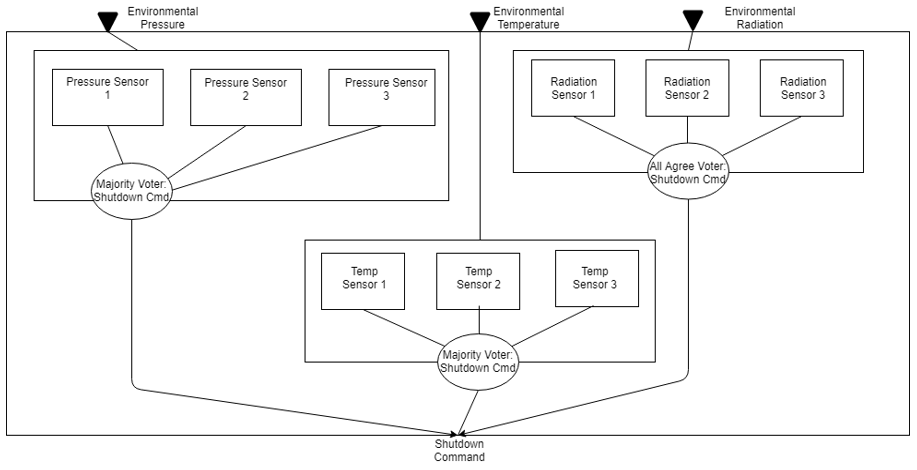
\includegraphics[width=0.6\textwidth]{images/sensorSys.PNG}
	\end{center}
	\vspace{-1em}
	\caption{Pressurized Water Reactor Sensor System}
	\label{fig:sensorSys}
	%\vspace{-2em}
\end{figure*}

\subsection{PWR Nominal Model}
The ``top-level" system is an abstraction of the PWR and contains sensor subsystems. The subsystems contain sensors that monitor pressure, temperature, and radiation. Environmental inputs are fed into each sensor in the model and the redundant sensors monitor temperature, pressure, or radiation respectively. If temperature, pressure, or radiation is too high, a shut down command is sent from the sensors to the parent components. 

The temperature, pressure, and radiation sensor subsystems use a voting mechanism on the redundant sensor values and will send a shut down command based on this output. The safety property of interest in this system is: \emph{shut down when and only when we should}; the AGREE guarantee stating this property is shown in Figure~\ref{fig:shutdownGuar}. 

\begin{figure*}[h!]
	%\vspace{-2em}
	\begin{center}
		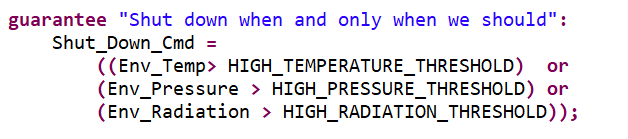
\includegraphics[width=0.5\textwidth]{images/sensorGuar.PNG}
	\end{center}
	\vspace{-2em}
	\caption{Sensor System Safety Property}
	\label{fig:shutdownGuar}
	%\vspace{-2em}
\end{figure*}

The safety of the system requires a shut down to take place if the temperature, pressure, or radiation levels become unsafe; thus, a threshold is introduced and if any sensor subsystem reports passing that threshold, a shutdown command is sent. But on the other hand, we do not want to shut down the system if it is not necessary. If a sensor reports high temperature erroneously and a shut down occurs, this costs time and money. 

Supporting guarantees are located in each sensor subsystem and correspond to temperature, pressure, and radiation sending a shut down command if sensed inputs are above a given threshold. Each sensor has a similar guarantee. 

\subsection{PWR Fault Model}
The faults that are of interest in this example system are any one of the sensors failing high or low. If sensors report high and a shut down command is sent, we shut down when we should not. On the other hand, if sensors report low when it should be high, a shut down command is not sent and we do not shut down when we should. For the remainder of this example, we focus on the failures when sensors report low when they should not.

Two faults are defined with the safety annex for each sensor in the system. An example of a temperature sensor fault stuck at high is shown in Figure~\ref{fig:tempSensorFault}.

\begin{figure*}[h!]
	\vspace{-2em}
	\begin{center}
		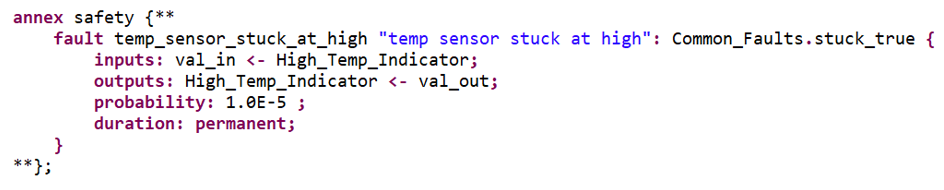
\includegraphics[width=0.8\textwidth]{images/tempSensorFault.PNG}
	\end{center}
	\vspace{-2em}
	\caption{Fault on Temperature Sensor Defined in the Safety Annex for AADL}
	\label{fig:tempSensorFault}
	\vspace{-2em}
\end{figure*}

The Safety Annex provides a way to weave the faults into the nominal model by use of the \emph{inputs} and \emph{outputs} keywords. This allows users to define a fault and attach it to the output of a component. If the fault is active, the error can then in essence violate the guarantees of this component and possibly the assumptions of downstream components~\cite{stewart2020safety}. The activation of a fault is not up to the user, but instead left up to the backend model checker, JKind, to determine if the activation of this fault will contribute to a violation of higher level guarantees. If so, it can be activated during the analysis.

For simplicity, throughout this paper we refer only to faults that fail low (i.e., the environmental input is actually high which warrants a shut down command, but the sensor reports that it is within safe ranges). This simplification is presented to keep the example and results described concise. For ease of reference, a table is provided giving model elements of interest in the sensor example. We refer to these throughout this section. Note: the thresholds vary for pressure, temperature, and radiation. These are given as constants $T_p$, $T_t$, and $T_r$ respectively. The shutdown command is defined notationally as $S$.  The faults are shown as ``fail low" which correspond to the temp (or pressure or radiation) being high, but the sensor reports safe ranges. We also do not list all guarantees and assumptions that are in the model, but only the ones of interest for this analysis. \danielle{Still messing around with how to display this in a way that it isn't messy, doesn't take up a ton of space, and am not currently happy with this approach. But I really hated the tables. Too much info for what is actually needed. Will keep working on this.}

\begin{description}[parsep=0.3ex]
 \item[PWR System:] $P = ((temp$ $>$ $T_t)$ $\lor$ $ (pressure$ $>$ $ T_p)$  $\lor$ $ (radiation$ $>$ $ T_r)) \iff S$\\
 \item[Temp Subsystem]: $G_t = temp$ $>$ $ T_t \iff S$\\
 \item[Pressure Subsystem:] $G_p = pressure$ $>$ $ T_p \iff S$\\
 \item[Radiation Subsystem:] $G_r = radiation$ $>$ $ T_r \iff S$\\
 \item[Temp Sensors (3):] $g_p = pressure$ $>$ $ T_p \iff S$, Fault $f_{ti}$: fails low for $i = 1, 2, 3$.\\
\item[Pressure Sensors (3):] $g_r = radiation$ $>$ $ T_r \iff S$, Fault $f_{pi}$: fails low for $i = 1, 2, 3$. \\
 \item[Radiation Sensors (3):] $g_r = radiation$ $>$ $ T_r \iff S$, Fault $f_{ri}$: fails low for $i = 1, 2, 3$\\
 \end{description}


\begin{comment}
\begin{center}
\resizebox{0.5\textwidth}{!}{%
    \begin{tabular}{ | c | c | c |}
      \hline
      \thead{Component} & \thead{Layer of Analysis} & \thead{Guarantee}\\
      \hline
      ReactorSys & Top &  \makecell{Safety Property $P$: \\ $((temp$ $>$ $T_t)$ $\lor$ $ (pressure$ $>$ $ T_p)$  $\lor$ $ (radiation$ $>$ $ T_r))$ \\ $\iff SHUTDOWN$}    \\
      \hline
      TempSys & Leaf  &  \makecell{Guarantee $G_t$: \\  $temp$ $>$ $ T_t \iff SHUTDOWN$}   \\
      \hline
      PressureSys & Leaf  &  \makecell{Guarantee $G_p$: \\ $pressure$ $>$ $ T_p \iff SHUTDOWN$}    \\
	\hline
      RadiationSys & Leaf  &  \makecell{Guarantee $G_r$: \\ $radiation$ $>$ $ T_r \iff SHUTDOWN$}   \\
      \hline
    \end{tabular}}
  \end{center}

\begin{center}
\resizebox{0.5\textwidth}{!}{%
    \begin{tabular}{ | c | c | c |}
      \hline
      \thead{Component} & \thead{Layer of Architecture} & \thead{Faults}\\
      \hline
      Temp Sensors (3) & \makecell{Leaf \\ Components} & \makecell{$f_{t}$: fail low}  \\
      \hline
	Pressure Sensors (3) & \makecell{Leaf \\ Components} & \makecell{$f_{p}$: fail low}  \\
      \hline
	Radiation Sensors (3) & \makecell{Leaf \\ Components} & \makecell{$f_{r}$: fail low}  \\
      \hline
    \end{tabular}}
  \end{center}



\subsection{Using this Example in the Generation of Minimal Cut Sets}
Step by step, we outline how minimal cut sets are generated through the \aivcalg algorithm using the sensor system as an example. For ease of reference, a table is provided giving model elements of interest in the sensor example. We refer to these throughout this section. Note: the thresholds vary for pressure, temperature, and radiation. These are given as constants $T_p$, $T_t$, and $T_r$ respectively. We also do not list all guarantees and assumptions that are in the model, but only the ones of interest for this analysis.

\begin{center}
\resizebox{\textwidth}{!}{%
    \begin{tabular}{ | c | c | c |}
      \hline
      \thead{Component} & \thead{Layer of Analysis} & \thead{Guarantee}\\
      \hline
      ReactorSys & Top &  \makecell{Safety Property $P$: \\ $((temp$ $>$ $T_t)$ $\lor$ $ (pressure$ $>$ $ T_p)$  $\lor$ $ (radiation$ $>$ $ T_r))$ \\ $\iff SHUTDOWN$}    \\
      \hline
      TempSys & Leaf  &  \makecell{Guarantee $g_t$: \\  $temp$ $>$ $ T_t \iff SHUTDOWN$}   \\
      \hline
      PressureSys & Leaf  &  \makecell{Guarantee $g_p$: \\ $pressure$ $>$ $ T_p \iff SHUTDOWN$}    \\
	\hline
      RadiationSys & Leaf  &  \makecell{Guarantee $g_r$: \\ $radiation$ $>$ $ T_r \iff SHUTDOWN$}   \\
      \hline
    \end{tabular}}
  \end{center}

\begin{center}
%\resizebox{\textwidth}{!}{%
    \begin{tabular}{ | c | c | c |}
      \hline
      \thead{Component} & \thead{Layer of Architecture} & \thead{Faults}\\
      \hline
      Temp Sensors (3) & \makecell{Leaf \\ Components} & \makecell{$f_{t}$: fail low}  \\
      \hline
	Pressure Sensors (3) & \makecell{Leaf \\ Components} & \makecell{$f_{p}$: fail low}  \\
      \hline
	Radiation Sensors (3) & \makecell{Leaf \\ Components} & \makecell{$f_{r}$: fail low}  \\
      \hline
    \end{tabular}
  \end{center}

The first two steps of this process are performed top down in conjunction with JKind analysis over a program. Thus, the top layer is analyzed first, then the next and so on. Steps 3 and 4 proceed after all MIVCs for each layer have been generated. We walk through this sensor system example in this fashion. 

\textbf{Step 1a: Preprocessing top layer.} The preprocessing step inserts specific MIVC elements into the Lustre program. The MIVC elements are the model elements considered in the constraint system for a given property. The Safety Annex provides the means to define a fault over the output of a component. This fault is given an unassigned \emph{trigger} Boolean literal in Lustre. If the trigger literal is true, the output of the component is changed. If not, the output remains equivalent to the nominal output of this component~\cite{stewart2020safety, Stewart17:IMBSA}. This trigger in Lustre is called a \emph{fault activation literal}. The IVC elements required in order to perform this transformation are these fault activation literals as well as guarantees. The basic rules used to insert these additional literals into Lustre depend on the analysis layer of that is being formed in Lustre and are as follows. 
\begin{itemize}
\item Leaf layer of analysis: only fault activation literals are added.
\item Middle or top layers: guarantees are added and if a direct subcomponent is a leaf component of the architecture and faults are defined on its outputs, then these faults are also added.
\end{itemize}

At the top level, guarantees of the sensor subsystems are the IVC elements.
$$\boxed{g_t, g_p, g_r}$$

There are distinct constraint systems, one for each property being proved. In this system at the top layer, there is a single property $P$; this results in the following constraint system. 
$$\boxed{C = \{g_t, g_p, g_r, \neg P\}}$$

\textbf{Step 2a: Generate all MIVCs for the constraint system at the top layer.} In order to prove $P$, all three guarantees from the sensor subsystem level are required. 
$$\boxed{MIVC(P) = \{g_t, g_p, g_r\}}$$. 

\textbf{Step 1b: Preprocessing leaf layer.} Model elements for the IVC algorithm consideration are the faults for each sensor, for instance temperature sensors:
$$\boxed{f_{t1}, f_{t2}, f_{t3}}$$ 

The resulting constraint system for the temperature sensor subsystem layer is:
$$\boxed{C = \{\neg f_{t1}, \neg f_{t2}, \neg f_{t3}, \neg g_t\}}$$

\textbf{Step 2b: Generate all MIVCs for the constraint system at the leaf layer.} Due to the majority voting mechanism, the MIVCs show all possible pairs of faults restricted to \emph{false}. This means, if any combination of two faults do not occur, then the guarantees at the temperature sensor subsystem level are satisfied. 
$$\boxed{
	\begin{aligned}
		MIVC_1(g_t) = \{\neg f_{t1}, \neg f_{t2}\} \\
		MIVC_2(g_t) = \{\neg f_{t1}, \neg f_{t3}\} \\
		MIVC_3(g_t) = \{\neg f_{t2}, \neg f_{t3}\}
	\end{aligned}
}$$

At this point, all MIVCs have been successfully generated (which is a requirement of the following algorithms) and we can move on to the generation of minimal cut sets. 

\textbf{Step 3a: Generate MCSs using a hitting set algorithm at the top layer.} Our single MIVC in this case will reveal three associated MCSs. (Notice: $MCS_1 \cap MIVC(P) \neq \emptyset$, and same for $MCS_2$ and $MCS_3$, thus these are hitting sets.)
 $$\boxed{
	\begin{aligned}
		MCS_1(top) = \{g_t\} \\
		MCS_2(top) = \{g_p\} \\
		MCS_3(top) = \{g_r\}
	\end{aligned}
}$$

\textbf{Step 4a: Transform MCSs into MinCutSets at the top layer.} Given that only guarantees are found in the MCSs at this layer, recursion is used to find the faults that cause violation of these guarantees. Using this recursion on $MCS_1$, we show the process further. 

\textbf{Step 3b: Generate MCSs using a hitting set algorithm at the leaf layer.} In step 2b, we found all MIVCs for the contract $g_t$ and send these to the hitting set algorithm. The resulting MCSs are: 
 $$\boxed{
	\begin{aligned}
		MCS_1(leaf) = \{\neg f_{t1}, \neg f_{t2}\} \\
		MCS_2(leaf) = \{\neg f_{t1}, \neg f_{t3}\} \\
		MCS_3(leaf) = \{\neg f_{t2}, \neg f_{t3}\}
	\end{aligned}
}$$

Only constrained faults are found in these MCSs, so we simply remove those constraints and have found the MinCutSets for the contracts $g_t$. These are returned and replace this contract in the top layer $MCS_1(top)$. Here is the end result for $MCS_1(top)$; this can be understood as three of the total minimal cut sets for $P$. 

\begin{equation*}
MCS_1(top) \rightarrow \left\{ \,
\begin{IEEEeqnarraybox}[][c]{l?s}
\IEEEstrut
MinCutSet_1(P) = \{f_{t1}, f_{t2}\}, \\
MinCutSet_2(P) = \{f_{t1},  f_{t3}\}, \\
MinCutSet_3(P) = \{f_{t2}, f_{t3}\}
\IEEEstrut
\end{IEEEeqnarraybox}
\right.
\end{equation*}

After all replacements have been made, we are left with all minimal cut sets for the property of interest ($P$ in this example). 

\end{comment}











\section{Preliminaries for Minimal Cut Set Generation}
\label{sec:prelimMCS}
In this research we consider \emph{safety properties} over infinite-state machines. The states are vectors of variables that define the values of state variables. We assume there are a set of legal \emph{initial states} and the safety property is specified as a formula over state variables. A \emph{reachable state space} means that all states are reachable from the initial state. 

Given a state space $U$, a transition system $(I,T)$ consists of an
initial state predicate $I : U \to \bool$ and a transition step
predicate $T : U \times U \to \bool$.
We define the notion of
reachability for $(I, T)$ as the smallest predicate $\reach : U \to
\bool$ which satisfies the following formulas:
\begin{gather*}
  \forall u.~ I(u) \Rightarrow \reach(u) \\
  \forall u, u'.~ \reach(u) \land T(u, u') \Rightarrow \reach(u')
\end{gather*}
A safety property $P : U \to \bool$ is a state predicate. A safety
property $P$ holds on a transition system $(I, T)$ if it holds on all
reachable states, i.e., $\forall u.~ \reach(u) \Rightarrow P(u)$,
written as $\reach \Rightarrow P$ for short. When this is the case, we
write $(I, T)\vdash P$.

\subsection{Induction}
For an arbitrary transition system $(I, T)$, computing reachability
can be very expensive or even impossible. Thus, we need a more
effective way of checking if a safety property $P$ is satisfied by the
system. The key idea is to over-approximate reachability. If we can
find an over-approximation that implies the property, then the
property must hold. Otherwise, the approximation needs to be refined.

A good first approximation for reachability is the property itself.
That is, we can check if the following formulas hold:
\begin{gather}
  \forall s.~ I(s) \Rightarrow P(s)
  \label{eq:1-ind-base} \\
  \forall s, s'.~ P(s) \land T(s, s') \Rightarrow P(s')
  \label{eq:1-ind-step}
\end{gather}
If both formulas hold then $P$ is {\em inductive} and holds over the
system. If (\ref{eq:1-ind-base}) fails to hold, then $P$ is violated
by an initial state of the system. If (\ref{eq:1-ind-step}) fails to
hold, then $P$ is too much of an over-approximation and needs to be
refined.

The JKind model checker used in this research uses {\em
  $k$-induction} which unrolls the property over $k$ steps of the
transition system. For example, 1-induction consists of formulas
(\ref{eq:1-ind-base}) and (\ref{eq:1-ind-step}) above, whereas
2-induction consists of the following formulas:
\begin{gather*}
\forall s.~ I(s) \Rightarrow P(s) \\
\forall s, s'.~ I(s) \land T(s, s') \Rightarrow P(s') \\
\forall s, s', s''.~ P(s) \land T(s, s') \land P(s') \land T(s',
  s'') \Rightarrow P(s'')
\end{gather*}
That is, there are two base step checks and one inductive step check.
In general, for an arbitrary $k$, $k$-induction consists of $k$
base step checks and one inductive step check as shown in
Figure~\ref{fig:k-induction} (the universal quantifiers on $s_i$ have
been elided for space). We say that a property is $k$-inductive if it
satisfies the $k$-induction constraints for the given value of $k$.
The hope is that the additional formulas in the antecedent of the
inductive step make it provable.

\begin{figure}
\begin{gather*}
I(s_0) \Rightarrow P(s_0) \\[-2pt]
%
\vdots \\[2pt]
%
I(s_0) \land T(s_0, s_1) \land \cdots \land T(s_{k-2}, s_{k-1})
\Rightarrow P(s_{k-1}) \\[2pt]
%
P(s_0) \land T(s_0, s_1) \land \cdots \land P(s_{k-1}) \land
T(s_{k-1}, s_k) \Rightarrow P(s_k)
\end{gather*}
\caption{$k$-induction formulas: $k$ base cases and one inductive
  step}
\label{fig:k-induction}
\end{figure}

In practice, inductive model checkers often use a combination of the
above techniques. Thus, a typical conclusion is of the form ``$P$ with
lemmas $L_1, \ldots, L_n$ is $k$-inductive''.

\subsection{The SAT Problem}
Boolean Satisfiability (SAT) solvers attempt to determine if there exists a total truth assignment to a given propositional formula, that evaluates to TRUE. Generally, a propositional formula is any combination of the disjunction and conjunction of literals (as an example, $a$ and $\neg a$ are literals). For a given unsatisfiable problem, solvers try to generate a proof of unsatisfiability; this is generally more useful than a proof of satisfiability. Such a proof is dependent on identifying a subset of clauses that make the problem unsatisfiable (UNSAT). 

SAT solvers in model checking work over a constraint system to determine satisfiability. A \textit{constraint system} $C$ is an ordered set of $n$ abstract constraints $\{C_1, C_2, ..., C_n\}$ over a set of variables. The constraint $C_i$ restricts the allowed assignments of these variables in some way~\cite{liffiton2016fast}. Given a constraint system, we require some method of determining, for any subset $S \subseteq C$, whether $S$ is \textit{satisfiable} (SAT) or \textit{unsatisfiable} (UNSAT). When a subset $S$ is SAT, this means that there exists an assignment allowed by all $C_i \in S$; when no such assignment exists, $S$ is considered UNSAT. 

There are several ways of translating a propositional formula into clauses such that satisfiability is preserved~\cite{een2003temporal}. By performing this translation, $k$-inductive model checkers are able to utilize parallel SAT-solving engines to glean information about the proof of a safety property at each inductive step. Expression of the base and induction steps of a temporal induction proof as SAT problems is straightforward. As an example, we look at an arbitrary base case from Figure~\ref{fig:k-induction}.

\begin{gather*}
I(s_0) \land T(s_0, s_1) \land \cdots \land T(s_{k-2}, s_{k-1})
\land \neg P(s_{k-1})
\end{gather*}

When proving correctness it is shown that the formulas are \emph{unsatisfiable}. If an $n^{th}$ inductive-step is unsatisfiable, that means following an $n$-step trace where the property holds, there exists no next state where it fails, i.e., the property $P$ is provable.





\section{Formalization of the Method}
\label{sec:formMCS}
\danielle{Section desperately needs figures of some kind to break up the text. Will try to make a few small ones of PWR example results.}
Compositional analysis proceeds from the top layer of the architecture down through the system model; faults are defined on leaf level components and guarantees are defined on all components. Due to the difference in analysis per layer, this section focuses on the formalism per layer type we are in. 

Given an initial state $I$ and a transition relation $T$ consisting of conjunctive constraints as defined in section~\ref{sec:prelim}. The nominal guarantees of the system, $G$, consist of conjunctive constraints $g \in G$. Given no faults, each $g$ is one of the transition constraints $T_i$ where:

\begin{gather}
T_n = g_1 \land  g_2 \land \cdots \land g_n
\label{eq:Tn}
\end{gather}

We assume the property holds of the nominal relation $(I,T_n) \vdash P$. Given that our focus is on safety analysis in the presence of faults, let the set of all faults in the system be  denoted as $F$. A fault $f \in F$ is a deviation from the normal constraint imposed by a guarantee. Any ``faults" in a mid-layer are simply violated guarantees, or deviations from normal behavior.

\subsection{Top Layer of Compositional Analysis}
Since faults are defined at leaf layers of the architecture, the top (and middle) layers only contain guarantees in the analysis. The \aivcalg algorithm collects all {\em minimal unsatisfiable subsets} (MUSs) of a given transition system in terms of the \textit{negation} of the top level property~\cite{Ghassabani2017EfficientGO,bendik2018online}. Formally, an MUS of a constraint system $C$ is a set $M \subseteq C$ such that $M$ is unsatisfiable and $\forall c \in M$ : $M \setminus \{c\}$ is satisfiable. The MUSs are the minimal explanation of the infeasibility of this constraint system; equivalently, these are the minimal sets of model elements necessary for proof of the safety property.

Returning to our running example, this can be illustrated by the following. Given the constraint system $C = \{G_p, G_t, G_r, \neg P\}$, a minimal explanation of the infeasability of this system is the set $\{G_p, G_t, G_r,\}$. If all three guarantees hold, then $P$ is provable. 

A related set is a {\em minimal correction set} (MCS); a MCS $M$ of a constraint system $C$ is a subset $M\subseteq C$ such that $C \setminus M$ is satisfiable and $\forall S \subset M$ : $C \setminus S$ is unsatisfiable. A MCS can be seen to ``correct'' the infeasability of the constraint system by the removal from $C$ the constraints found in an MCS.

In the case of an UNSAT system, we may ask: what will correct this unsatisfiability? Returning to the PWR example, we can find the MCSs of the top level constraint system: $MCS_1 = \{G_t\}$, $MCS_2 = \{G_p\}$, $MCS_3 = \{G_r\}$. If any single guarantee is violated, a shut down from that subsystem will not get sent when it should and the safety property $P$ will be violated. 

A duality exists between the MUSs of a constraint system and the MCSs as established by Reiter \cite{reiter1987theory}. This duality is defined in terms of \textit{Minimal Hitting Sets} (\textit{MHS}). A hitting set of a collection of sets $A$ is a set $H$ such that every set in $A$ is ``hit'' by $H$; $H$ contains at least one element from every set in $A$. Every MUS of a constraint system is a minimal hitting set of the system's MCSs, and likewise every MCS is a minimal hitting set of the system's MUSs~\cite{liffiton2016fast, reiter1987theory, de1987diagnosing}.

For the PWR top level constraint system, it can be seen that each of the MCSs intersected with the MUS is nonempty. And now we have the minimal set of guarantees for which, if violated, will cause $P$ to be unprovable. 

\subsection{Leaf Layer of Compositional Analysis}
The faults in the safety annex are defined on leaf level components. Thus, for the lowest analysis layer, we must take into consideration faults and the guarantees their activation may violate. A fault $f \in F$ is a deviation from the normal constraint imposed by a guarantee. For the purposes of this paper, each guarantee at the leaf layer of analysis has an associated fault. Without loss of generality, we associate a single fault and an associated fault probability with a guarantee. Each fault $f_i$ is associated with an \emph{activation literal}, $af_i$, that determines whether the fault is active or inactive. 

To consider the system under the presence of faults, consider a set $GF$ of modified guarantees in the presence of faults and let a mapping be defined from activation literals $af_i \in AF$ to these modified guarantees $gf_i \in GF$. 
\begin{center}
$\sigma : AF \rightarrow GF$ \\
$gf_i = \sigma(af_i) =$ if $af_i$ then $f_i$ else $g_i$
\label{eq:sigma}
\end{center}

The transition system is composed of the set of modified guarantees $GF$ and a set of conjunctions assigning each of the activation literals $af_i \in AF$ to false: 

\begin{gather}
T = gf_1 \land gf_2 \land \cdots \land gf_n \land \neg af_1 \land \neg af_2 \land \cdots \land \neg af_n
\label{eq:T}
\end{gather}

\begin{lemma} If $(I,T_n) \vdash P$ for $T_n$ defined in equation~\ref{eq:Tn}, then $(I,T) \vdash P$ for $T$ defined in equation~\ref{eq:T}.
\begin{proof}
By application of successive evaluations of $\sigma$ on each constrained activation literal $\neg af_i$, the result is immediate.
\end{proof}
\end{lemma}

Consider the elements of $T$ as a set $GF \cup AF$, where $GF$ are the potentially faulty guarantees and $AF$ consists of the activation literals that determine whether a guarantee is faulty. This is a set that is considered by a SAT-solver for satisfiability during the $k$-induction procedures. The posited problem is thus: $GF \land AF \land \neg P$ for the safety property in question. Recall, if this is an \emph{unsatisfiable} constraint system, then $(I,T) \vdash P$. On the other hand, if it is \emph{satisfiable}, then we know that given the constraints in $GF$ and $AF$, $P$ is not provable. These are the exact constraints we wish to find. 

Let us view this in terms of the PWR system example and focus on the temperature sensor subsystem. The safety property to be proved is $G_t$, the supporting guarantees are found in each of the three temperature sensors, $g_{ti}$. Faults $f_{ti}$ are defined for each sensor. The transition system is: 
\begin{gather*}
T = gf_{t1} \land gf_{t2} \land gf_{t3}  \land \neg af_{t1} \land \neg af_{t2} \land \neg af_{t3}
\end{gather*}

The MIVCs for this subsystem layer correspond to all pairwise combinations of constrained activation literals. Intuitively, if any two sensor faults do {\em not} occur, then two of the three sensor guarantees are not violated and the system responds appropriately to high temperature; therefore, $G_t$ is provable. 

The MCSs for this subsystem layer happen to also correspond to all pairwise combinations of constrained activation literals. If any two sensor faults {\em do} occur, then two of the three sensor guarantees will be violated and the system does not respond to high temperature as required. This would result in the inability to prove $G_t$. (Note: it is not always the case that the MCSs are the same as the MIVCs -- in this case it is due to majority voting on three sensors.)

\subsection{Transforming MCS into Minimal Cut Set}
The MCSs contain the information needed to find minimal cut sets, but their elements consist of constrained activation literals and/or guarantees. The link between the activation literals, faults, and guarantees is defined through $\sigma$ mapping (equation~\ref{eq:sigma}). At the leaf layer, only activation literals are found in MCSs and $\sigma$ must be applied to each element in an MCS to map back to the associated fault. Without loss of generality, let $MCS = \{af_1, \cdots, af_m\}$. Let $\sigma (MCS) = \{\sigma (\neg af_{1}), \cdots, \sigma (af_{m})\}$ be a mapping where MCS is a minimal correction set with regard to some property $G$ and $MCS  \subseteq AF$. \danielle{Question: Does minimality need its own proof?}

\begin{lemma} $\sigma (MCS)$ is a minimal cut set of $G$. 
\begin{proof}
Assume towards contradiction that $\sigma (MCS)$ is not a cut set of $G$. Then $gf_1 \land \cdots \land gf_n \land af_1 \cdots \land af_m \land \neg af_{k+1} \land \neg af_n \land \neg G$ is unsatisfiable. Thus, the \emph{true} activation literals do not affect the provability of $G$. This contradicts $C \setminus MCS$ is satisfiable. 
Minimality follows directly from the definition of MCS.
\end{proof}
\end{lemma}

In terms of the PWR example, the minimal cut sets for the temperature subsystem property $G_t$ consist of all pairwise faults on the temperature sensors; if any two faults occur on the sensors at the same time, we violate the temperature subsystem guarantee. 

Once these lower level minimal cut sets are generated, it is a matter of simple set replacement to find the higher level minimal cut sets. This can be easily seen in our example. An MCS at the top level has the element $G_t$. We systematically replace the contract with the faults that cause their violation. This results in three distinct minimal cut sets for $P$ from the temperature subsystem: $\{f_{t1}, f_{t2}\}, \{f_{t1}, f_{t3}, \{f_{t2}, f_{t3}$. All minimal cut sets for $P$ are given as similar pairwise combinations from each subsystem and total 9 for the entire system.

\danielle{Seems I need a theorem to round it out: that replacement will give min cut sets of safety property. Will think about how to formulate this.}




\section{Implementation and Algorithms}
\label{sec:algs}
The implementation of this idea requires changing what information the \aivcalg algorithm uses to complete the proofs and generate MUSs. At each layer of analysis, the \aivcalg algorithm views the model as a constraint system consisting of the negation of the property in question (guarantees at lower levels, top-level properties at the highest level), and the supporting guarantees/assumptions from the direct child level. The information provided to this algorithm changes slightly when performing the minimal cut set algorithms.

\subsubsection{Implementation}
In this approach, we use the all MIVCs algorithm and provide it a constraint system consisting of the negation of the top level safety property, the contracts of system components, as well as the faults in each layer constrained to false. It then collects the MUSs of this constraint system.

\begin{figure}[htbp]
	\hspace*{-2cm}
	\vspace{-0.1in} 
	\begin{center}
		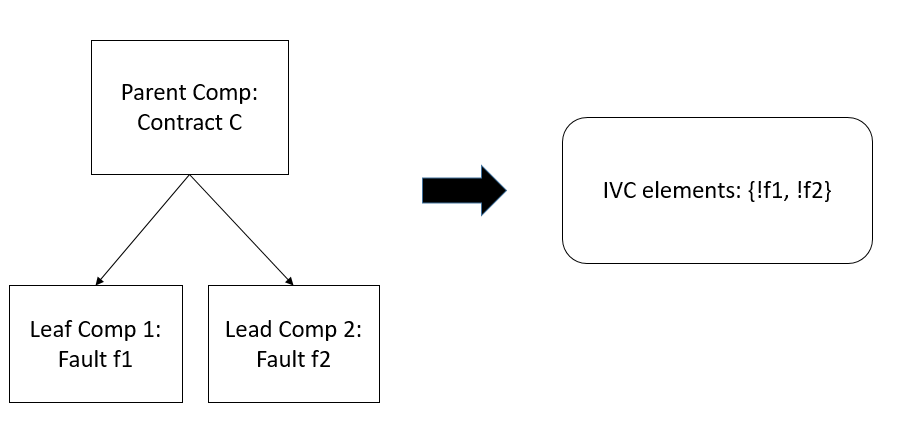
\includegraphics[scale=0.5]{images/ivcElements1.png}
	\caption{IVC Elements used for Consideration in a Leaf Layer of a System}
		\label{fig:ivcElements1}
	\end{center}
\end{figure}

Different layers of the architecture (and hence proof) provide slightly different information to the \aivcalg algorithm. This is ``given" to the IVC algorithm by the insertion of a Lustre statement with the keyword \texttt{\%IVC} followed by the fault activation literal. \\ \texttt{--\%IVC \_\_fault\_\_independently\_\_active\_\_sensor}\\

The constraints on that literal are given through the use of an assert statement in Lustre.\\ \texttt{assert (\_\_fault\_\_independently\_\_active\_\_sensor = false)}\\

The leaf nodes contribute only constrained faults to the IVC elements as shown in Figure~\ref{fig:ivcElements1}. In the non-leaf layers of the program, both contracts and constrained faults are considered as shown in Figure~\ref{fig:ivcElements2}. The reason for this is that the contracts are used to prove the properties at the next highest level and are necessary for the verification of the properties. The faults are used to provide safety pertinant information for the minimal cut sets. 

\begin{figure}[htbp]
	\hspace*{-2cm}
	\vspace{-0.1in} 
	\begin{center}
		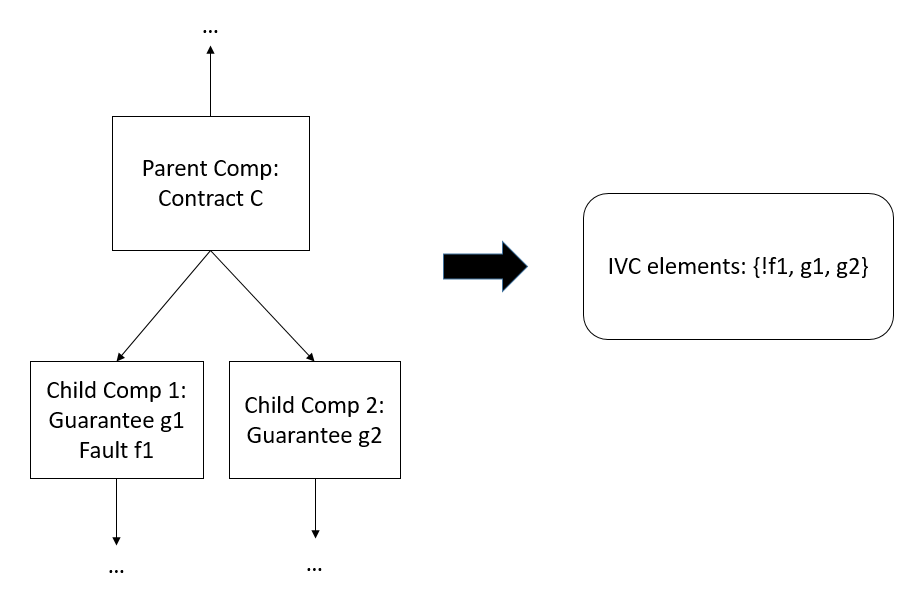
\includegraphics[scale=0.5]{images/ivcElements2.png}
	\caption{IVC Elements used for Consideration in a Middle Layer of a System}
		\label{fig:ivcElements2}
	\end{center}
\end{figure}

The all MIVCs algorithm returns the minimal set of these elements necessary to prove the properties. This equates to any contracts or inactive faults that must be present in order for the verification of properties in the model. From here, we perform a number of algorithms to transform all MIVCs into minimal cut sets.


%%%%%%%%%%%%%%%%%%%%%%%%%%%%%%%%%%%%%%%%%%%%%%%%%
%%%%%%%%%%%%%%%%%%%%            ALGORITHM DETAILS
\subsubsection{Algorithms}
The generation of \textit{MIVCs} traverses the program in a top down fashion. Likewise, the transformation of \textit{MIVCs} to MinCutSets traverses this program layer by layer if and only if all MIVCs have been generated. It is a requirement of the minimal hitting set algorithm that \textit{all} MUSs are used to find the MCSs~\cite{liffiton2016fast,gainer2017minimal,murakami2013efficient}. Thus, once all the MIVCs have been found and the minimal hitting set algorithm has completed, %our 
the MinCutSet Generation algorithm can begin. 

The MinCutSet Generation Algorithm begins with a list of MCSs specific to a top level property. These MCSs may contain a mixture of fault activation literals constrained to \textit{false} and %\textit{true} subcomponent contracts.
and subcomponent contracts constrained to \textit{true}. We remove all constraints from each MCS and call the resulting sets $I$, for \textit{Intermediate} set. Replacement of subcomponent contracts with their respective minimal cut sets can then proceed. For each of those contracts in $I$, we check to see if we have previously obtained a MinCutSet for that contract. If so, replacement is performed. If not, we recursively call this algorithm to obtain the list of all MinCutSets associated with this subcomponent contract. At a certain point, there will be no more contracts in the set $I$ in which case we have a minimal cut set for the current property. When this set is obtained, we store it in a lookup table keyed by the given property that this $I$ is associated with. 

A small example will illustrate this process. \danielle{Do I want to have a more concrete example? If so, pull from thesis proposal sensor example. If a shorter more abstract example is okay, do that.}







Algorithm~\ref{alg:generation_alg} describes this process.


\begin{algorithm}[htbp]
\SetKwFunction{FMain}{replace}
 \SetKwProg{Fn}{Function}{:}{}

	\Fn{\FMain{$P$}}{
		$List(I)$:= $List(MCS)$ for $P$ with all constraints removed \;
		\For{all $I \in List(I)$}{
			\eIf{there exists contracts $g \in I$}{
				\For{all constrained contracts $g \in I$}{
					\eIf{there exists $MinCutSets$ for $g$ in lookup table}{
						\For{all $minCut(g)$}{
							$I_{repl} = I$ \;
							$I_{repl} :=$ replace $g$ with $minCut(g)$ \;
							add $I_{repl}$ to $List(I)$ \;
						} %end for all cut sets of g
					}{
						replace($g$) \;
					} % end else if no cut sets in lookup table
				} % end for all constrained contracts in I
			}{
				add $I$ as $minCut(g)$ for $P$ \;
			} %end else if there exists contracts in I
		}%end for all I in list(I)
	}
%	\caption{Minimal Cut Set Generation Algorithm}
	\caption{MinCutSets Generation Algorithm}
	\label{alg:generation_alg}
\end{algorithm}

The number of replacements $R$ that are made in this algorithm are constrained by the number of minimal cut sets there are 
for all $\alpha$ contracts within the initial MCS. 

We call the set of all minimal cut sets for a contract $g$: $Cut(g)$. The following formula defines an upper bound on the number of replacements. The validity of this statement follows directly from the general multiplicative combinatorial principle. The number of replacements $R$ is bounded by the following formula:
\begin{equation}
\label{eq:bound}
  R \leq {\displaystyle \sum_{i=1}^{\alpha} }({\displaystyle \prod_{j=1}^{i} |Cut(g_j)|})  
\end{equation}


It is also important to note that the cardinality of $List(I)$ is bounded, i.e. the algorithm terminates. Every new $I$ that is generated through some replacement of a contract with its minimal cut set is added to $List(I)$ in order to continue the replacement process for all contracts in $I$. Adding to this set requires proof regarding termination.
\begin{theorem}
Algorithm~\ref{alg:generation_alg} terminates
\begin{proof}
No infinite sets are generated by the \aivcalg or minimal hitting set algorithms~\cite{Ghassabani2017EfficientGO,murakami2013efficient}; therefore, every MCS produced is finite. Thus, every $MinCutSet$ of every contract $g$ is finite. Furthermore, a bound exists on the number of additional intermediate sets $I$ that are added to $List(I)$: \\
$|List(I)| \leq R$ (Equation~\ref{eq:bound}).
\end{proof}
\end{theorem}

The reason for this upper bound is that for a contract $g_1$ in MCS, we make $|Cut(g_1)|$ replacements and add the resulting lists to $List(I)$. Then we move to the next contract $g_2$ in $I$. We must additionally make $|Cut(g_1)| \times |Cut(g_2)|$ replacements and add all of these resulting lists to $List(I)$, and so on throughout all contracts. Through the use of basic combinatorial principles, we end with the above formula for the upper bound on the number of additional intermediate sets.


\subsubsection{Pruning to Address Scalability}
The MinCutSets are filtered during this process based on a fault hypothesis given before analysis begins. The Safety Annex provides the capability to specify a type of verification in what is called a \textit{fault hypothesis statement}. These come in two forms: maximum number of faults or probabilistic analysis. Algorithm~\ref{alg:generation_alg} is the general approach, but the implementation changes slightly depending on which form of analysis is being performed. This pruning improves performance and diminishes the problem of combinatorial explosions in the size of minimal cut sets for larger models. \\

\textbf{Max $N$ Analysis Pruning} This statement restricts the number of faults that can be independently active simultaneously and verification is run with this restriction present. For example, if a max 2 fault hypothesis is specified, two or fewer faults may be active at once. In terms of minimal cut sets, this statement restricts the cardinality of minimal cut sets generated.

If the number of faults in an intermediate set $I$ exceeds the threshold $N$, any further replacement of remaining contracts in that intermediate set can never decrease the total number of faults in $I$; therefore, this intermediate set is eliminated from consideration.\\

\textbf{Probabilistic Analysis Pruning} The second type of hypothesis statement restricts the cut sets by use of a probabilistic threshold. Any cut sets with combined probability higher than the given probabilistic threshold are removed from consideration. The allowable combinations of faults are calculated before the transformation algorithm begins; this allows for a pruning of intermediate sets during the transformation. If the faults within an intermediate set are not a subset of any allowable combination, that intermediate set is pruned from consideration and no further replacements are made. 


